%! suppress = MissingImport
% Preamble
%\documentclass[11pt]{article}
\documentclass[9pt,twocolumn,twoside, lineno]{jost-new}

\templatetype{joststandard}

\numberwithin{subsection}{section}

% Packages
%\usepackage{amsmath}
%\usepackage{url}
\usepackage{subfig}
\usepackage{hyperref}

% Document
\title{MnDOT Traffic Capstone Report}
\shorttitle{MnDOT Capstone Report}
\author{Nathan Wodarz}
\leadauthor{Wodarz}
\begin{abstract}
\textbf{Abstract}: The state of Minnesota maintains over 140,000 miles of public roads, ranking fourth in the United
States.
The Minnesota Department of Transportation (MnDOT) has primary responsibility for planning, developing, and
maintaining state highways.
One of these responsibilities is tracking traffic volume on state roads and highways.
Using MnDOT counts from 2002 to present, we develop models for monthly traffic volume at over 100 different locations.
From these models, we obtain predictions for future traffic volumes.
\end{abstract}

\begin{document}
\maketitle
\thispagestyle{firststyle}
\ifthenelse{\boolean{shortarticle}}{\ifthenelse{\boolean{singlecolumn}}{\abscontentformatted}{\abscontent}}{}
\begin{nolinenumbers}
\tableofcontents
\end{nolinenumbers}
\pagebreak

%%%%%%%%%%%%%%%%%%%%%%%%%%%%%%%%%%%%%%%%%%%%%%%%%%%%%%%%%%%%%%%%%%%%%%%%%%%%%%%%%%%%%%%%%%%%%%%%%%%%%%%%%%%%%%%%%%%%%%%%
%%%%%%%%%%%%%%%%%%%%%%%%%%%%%%%%%%%%%%%%%%%%%%%%%% Introduction %%%%%%%%%%%%%%%%%%%%%%%%%%%%%%%%%%%%%%%%%%%%%%%%%%%%%%%%
%%%%%%%%%%%%%%%%%%%%%%%%%%%%%%%%%%%%%%%%%%%%%%%%%%%%%%%%%%%%%%%%%%%%%%%%%%%%%%%%%%%%%%%%%%%%%%%%%%%%%%%%%%%%%%%%%%%%%%%%

\section{Introduction}\label{sec:introduction}
The state of Minnesota ranks fourth out of the fifty states in the United States by two major measures.
In both, the state trails only Texas, California, and Illinois.
According to the most recent statistics available from the \href{https://www.fhwa.dot.gov/policyinformation/statistics/2019/}{Federal Highway Administration}\cite{fhwa}, Minnesota maintained 141,360 miles and 287,080 lane-miles of roads in 2019 (lane-miles are a measure of capacity - a four-lane road ten miles in length is 40 lane-miles).
The Minnesota Department of Transportation (MnDOT) is the agency responsible for overseeing the state's highway system.
MnDOT's mission statement indicates that its purpose is to "Plan, build, operate and maintain a safe, accessible, efficient and reliable multimodal transportation system that connects people
to destinations and markets throughout the state, regionally and around the world."\cite{mndot}

\subsection{Background}\label{subsec:background2}
As part of its responsibility, MnDOT tracks traffic volume throughout the state.
It has installed a series of \emph{automatic traffic recorders} (ATRs) throughout the state.
MnDOT says that over 155 devices are active, with at least 75  in the seven counties making up the Minneapolis-St. Paul metropolitan area and at least another 80 elsewhere in the state.
ATRs continuously track traffic, with some also being capable of detecting vehicle type and speed.
ATRs are often embedded in the road surface, although newer versions use radar and can be installed without requiring road closure.

Although technically different, MnDOT also uses \emph{Weigh-in-Motion} (WIM) devices to track the same data as ATRs. WIMs additionally track truck weights and configurations.
For the purposes of this study, WIM stations were considered the same as ATR stations.
All such stations will be referred to as ATRs for the remainder of this article.

\subsection{Problem Statement}\label{subsec:problem-statement}
We would like to develop a model which describes traffic volume at ATRs over the time covered by the data.
Additionally, we wish to make projections of future traffic volume over the remainder of the decade.

%%%%%%%%%%%%%%%%%%%%%%%%%%%%%%%%%%%%%%%%%%%%%%%%%%%%%%%%%%%%%%%%%%%%%%%%%%%%%%%%%%%%%%%%%%%%%%%%%%%%%%%%%%%%%%%%%%%%%%%%
%%%%%%%%%%%%%%%%%%%%%%%%%%%%%%%%%%%%%%%%%%%%%%%%%%%%%% Data %%%%%%%%%%%%%%%%%%%%%%%%%%%%%%%%%%%%%%%%%%%%%%%%%%%%%%%%%%%%
%%%%%%%%%%%%%%%%%%%%%%%%%%%%%%%%%%%%%%%%%%%%%%%%%%%%%%%%%%%%%%%%%%%%%%%%%%%%%%%%%%%%%%%%%%%%%%%%%%%%%%%%%%%%%%%%%%%%%%%%

\section{Data}\label{sec:data}
\subsection{Raw Data}\label{subsec:raw-data}
MnDOT provides a number of different data products related to its mission, including ATR reports.
These can be found at the \href{https://www.dot.state.mn.us/traffic/data/data-products.html}{MnDOT Data Products page}.
Data since 2017 is saved in .csv files.
These files contain one row per direction per station per day.
There is one entry for each hour of the day.
More recent files further subdivide station directions into lanes.
We are not concerned with lanes or directions, so we will ultimately aggregate into a single value per station.
Data prior to 2017 is also present on the website, although not indexed.
These are held in .txt reports, dating back to 2002.
The reports were located using the \href{https://archive.org/web/}{Wayback Machine} at the Internet Archive.
The .txt files contain the same information as the .csv files, but must be processed to access the information.

Along with the station counts, a file containing information on each active station was obtained from the Data Products page.
From this, we found information indicating whether each station was in a rural or urban location as well as the functional class of each road containing the stations.
The functional class shows a hierarchy of road types.
The classes used were "Interstates", "Principal Arterial - Other Freeways and Expressways", "Principal Arterial - Other", "Minor Arterial", "Major Collector", and "Local".
Interstates and other freeways (indicated in the class "Principal Arterial - Other Freeways and Expressways") are high speed limited-access multilane roads intended to move large volumes of traffic over distances.
Arterials (both major and minor) are regional.
They are higher volume roads and ideally have few intersections.
Their intent is to move traffic between freeways and collectors, which serve as mid-capacity roads.
Collectors then connect to local roads, which often serve residential neighborhoods.
Most stations were located in rural areas (Fig.~\ref{fig:urban_rural_pie}) and nearly half are located on arterials (Fig.~\ref{fig:functional_class_pie})
\begin{figure}[h!]
\centering
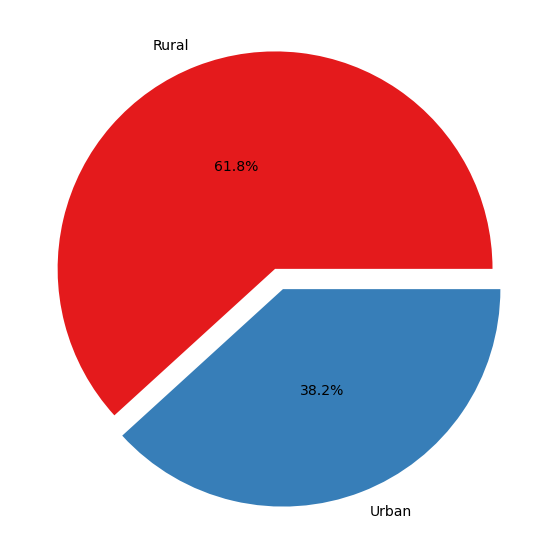
\includegraphics[width=\linewidth]{figures/urban_rural_pie.png}
\caption{Station Locations: Rural vs. Urban}
\label{fig:urban_rural_pie}
\end{figure}

\begin{figure}[h!]
\centering
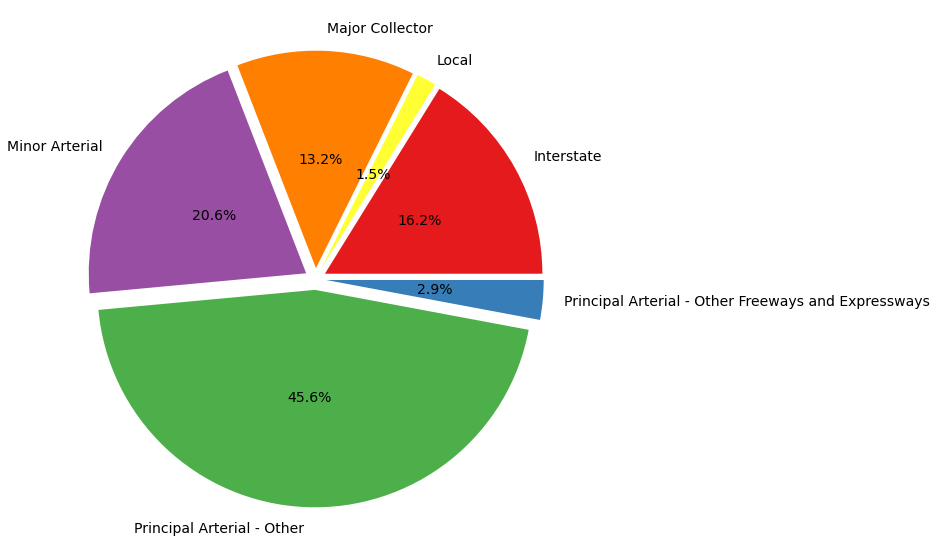
\includegraphics[width=\linewidth]{figures/functional_class_pie.png}
\caption{Station Functional Class}
\label{fig:functional_class_pie}
\end{figure}

\subsection{Cleaning}\label{subsec:cleaning}
While reading the .txt reports, some reports were found to be mislabeled.
These were corrected and resulting duplicate records were removed.
Direction and lane subtotals were aggregated hourly.

The standard method for reporting highway volumes is the Annual Average Daily Traffic (AADT).
The Federal Highway Administration recommends calculating the AADT as a weighted average of Monthly Average Daily Traffic (MADT) values, where the weights are the lengths of the months \cite{fhwa2}.
The MADT definition isn't quite the mean daily value, as definition is designed to remove bias from missing values and from differing numbers of weekdays in each month.
The MADT is given by the formula
\[
MADT_m = \frac{\sum_{j=1}^7 w_{jm} \sum_{h=1}^{24}\left[\frac{1}{n_{hjm}}\sum_{i=1}^{n_{hjm}}VOL_{ihjm}\right]}{\sum_{j=1}^7 w_{jm}}
\]
where $m$ is the month (represented as an integer between 1 and 12), $j$ is the day of the week (represented as an integer between 1 and 7), $h$ is the hour of the day (as an integer from 1 to 24), $w_{jm}$ is the number of times the $j$th day of the week occurs in month $m$, $n_{hjm}$ is the number of available data points for the $h$th hour of the $j$th day of the week in month $m$ (between 1 and 5), $VOL_{ihjm}$ is the $i$th data point for the $h$th hour of the $j$th day of the week in month $m$, and $MADT_m$ is the monthly average daily traffic for month $m$.
The particular choice of which day of the week and hour of the day are represented by 1 doesn't affect the result.
We replaced the hourly counts by the MADT according to this formula.

Next, we removed several stations.
Any inactive station was removed as well as stations reporting very little data.
Over a dozen stations have only been collecting from 2019 or later.
These stations have almost no data that can be used for training.
We dropped any station with 80\% or more missing MADT values in the range from January 2002 to July 2021.
We made two other adjustments.
Any station with no updates in the last 12 months was removed from the data set.
Finally, there were two stations containing a total of three non-null zero entries in the set of MADT values.
Examining the distributions for both stations, the zero values were found to be outliers.
We removed those entries as well.

%%%%%%%%%%%%%%%%%%%%%%%%%%%%%%%%%%%%%%%%%%%%%%%%%%%%%%%%%%%%%%%%%%%%%%%%%%%%%%%%%%%%%%%%%%%%%%%%%%%%%%%%%%%%%%%%%%%%%%%%
%%%%%%%%%%%%%%%%%%%%%%%%%%%%%%%%%%%%%%%%%%%% Exploratory Data Analysis %%%%%%%%%%%%%%%%%%%%%%%%%%%%%%%%%%%%%%%%%%%%%%%%%
%%%%%%%%%%%%%%%%%%%%%%%%%%%%%%%%%%%%%%%%%%%%%%%%%%%%%%%%%%%%%%%%%%%%%%%%%%%%%%%%%%%%%%%%%%%%%%%%%%%%%%%%%%%%%%%%%%%%%%%%

\section{Exploratory Data Analysis}\label{sec:exploratory-data-analysis}
\subsection{Distribution of Time Series}
Visually, we can see that the distributions of stations vary by functional class.
Interstates and other freeways carry a much larger number of vehicles than other roads.
We compare the distributions arising from interstate stations with those from minor arterials in Figs.~\ref{fig:hist_interstate} and \ref{fig:hist_minor_arterial}.

\begin{SCfigure*}[\sidecaptionrelwidth][h!]
\centering
    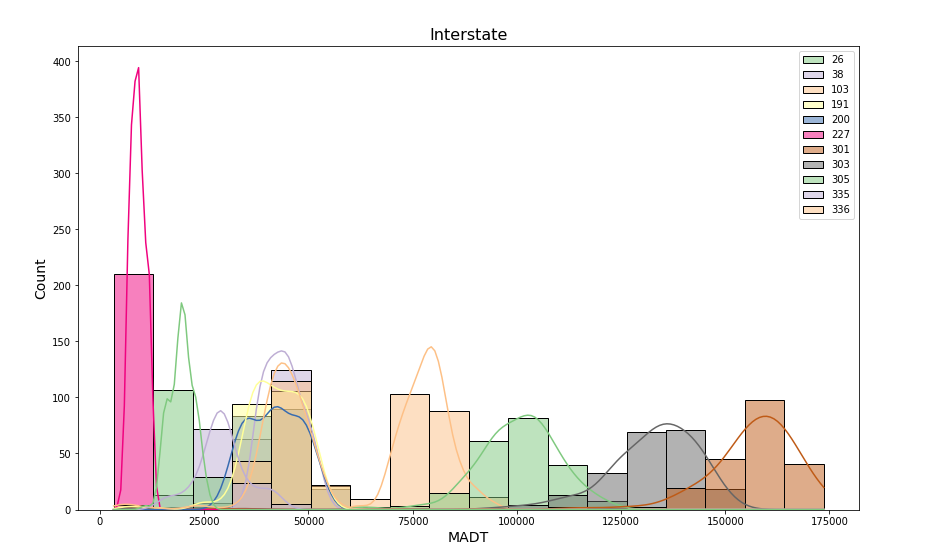
\includegraphics[width=14.4cm]{figures/hist_interstate.png}
\caption{MADT Distribution: Interstates}
\label{fig:hist_interstate}
\end{SCfigure*}
\begin{SCfigure*}[\sidecaptionrelwidth][h!]
\centering
    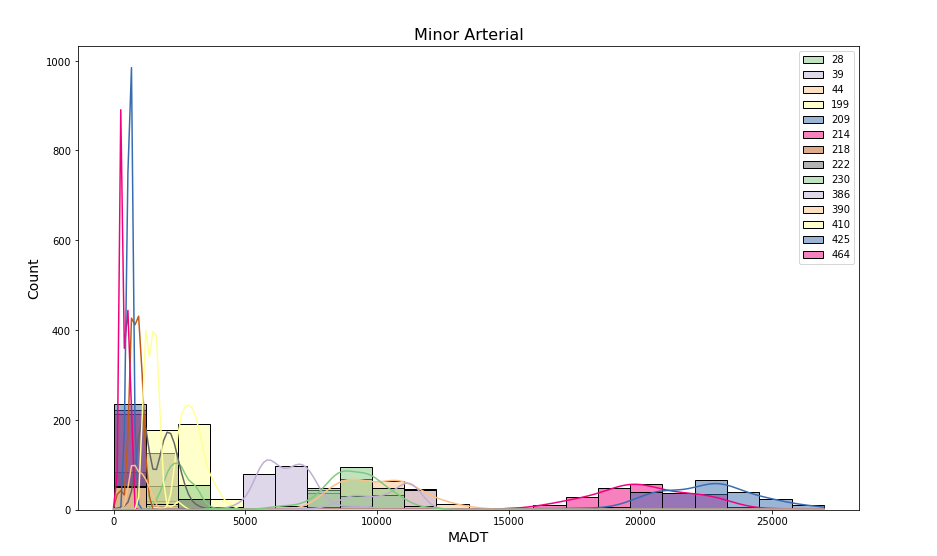
\includegraphics[width=14.4cm]{figures/hist_minor_arterial.png}
\caption{MADT Distribution: Interstates}
\label{fig:hist_minor_arterial}
\end{SCfigure*}

\subsection{Stationarity}
We performed both Augmented Dickey-Fuller and Kwiatkowski–Phillips–Schmidt–Shin (KPSS) tests to examine each time series for stationarity.
Despite the obvious presence of annual seasonality (a collection of auto-correlation function plots are shown in Fig.~\ref{fig:autocorrelations_a1}), the majority of time series were found to be stationary (and/or lacking a unit root) by both tests.
\begin{SCfigure*}[\sidecaptionrelwidth][h!]
\centering
    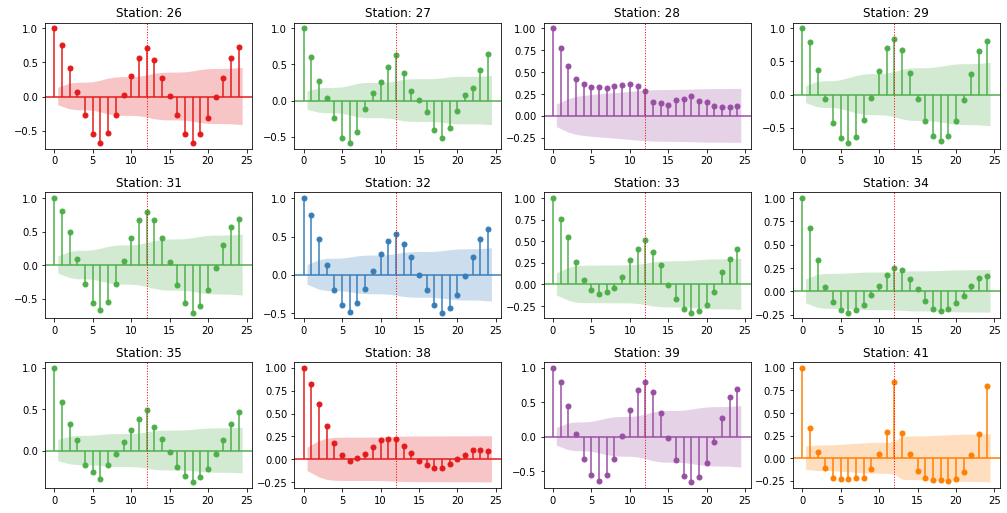
\includegraphics[width=14.4cm]{figures/autocorrelations_a1.png}
\caption{Sample of ACF Plots, Indicating Annual Seasonality}
\label{fig:autocorrelations_a1}
\end{SCfigure*}

We did not concern ourselves with the failure of the tests, as the model fitting did not require stationary models.
%%%%%%%%%%%%%%%%%%%%%%%%%%%%%%%%%%%%%%%%%%%%%%%%%%%%%%%%%%%%%%%%%%%%%%%%%%%%%%%%%%%%%%%%%%%%%%%%%%%%%%%%%%%%%%%%%%%%%%%%
%%%%%%%%%%%%%%%%%%%%%%%%%%%%%%%%%%%%%%%%%%%%%%%%%%%%% Modeling %%%%%%%%%%%%%%%%%%%%%%%%%%%%%%%%%%%%%%%%%%%%%%%%%%%%%%%%%
%%%%%%%%%%%%%%%%%%%%%%%%%%%%%%%%%%%%%%%%%%%%%%%%%%%%%%%%%%%%%%%%%%%%%%%%%%%%%%%%%%%%%%%%%%%%%%%%%%%%%%%%%%%%%%%%%%%%%%%%

\section{Modeling}\label{sec:modeling}
Evaluation of models was performed on a training set consisting of the counts corresponding to the first 80\% of
timestamps.
The last 20\%, which included the timestamps covered by the COVID-19 pandemic, were held out for testing purposes.
When required (for imputation and deep learning methods), a validation set was heldout from the training set.

\subsection{Imputation}\label{subsec:imputation}
There were a considerable number of missing data points.
While many of these could be attributed to stations that were installed well after 2002, many stations were missing one
or more months in the middle of the data.
As many time series methods don't work with missing values, we decided to impute all missing entries.
For validation purposes, 49\% of training set timestamps were held out.
The choice was made to hold values out uniformly at random from all timestamps in the training set to verify that the
imputation technique selected would successfully fill gaps in the middle of data.

There were three imputation methods tested, each with two variants.
We compared the six alternatives using mean square error.
Each time series was scaled to the interval $[0,1]$ before imputation and returned to the full scale after.
This was done so that the results would not be biased by a strong performance on a single time series.

The base methods we used were imputation with the mean, CDRec (Centroid Decomposition), and Facebook Prophet.
CDRec is a method developed by Khayati, Cudré-Mauroux, and Böhlen to impute values in correlated time series \cite{khayati}.
This was the only method tested that took correlations into account, as both the mean and Prophet work on each series independently.
Both the mean imputation and CDRec were done in a straightforward manner as well as partitioning the data into twelve components, one for each month of the year.
The plain methods were performed on each component and the resulting frames were re-assembled.
For Prophet, we examined both the default linear algorithm as well as the alternate logistic algorithm.

The base CDRec algorithm was able to capture some seasonality, but proved to be too conservative.
The seasonal CDRec variant proved to be the best-performing alternative (Fig.~\ref{fig:impute_mse}).
An example of the performance of CDRec on a single time series is shown in Fig.~\ref{fig:impute_seasonal_cdrec}.
The seasonal CDRec slightly outperformed imputing seasonally with the mean.
Neither of the Prophet variants behaved well in general.

\begin{SCfigure*}[\sidecaptionrelwidth][h!]
\centering
    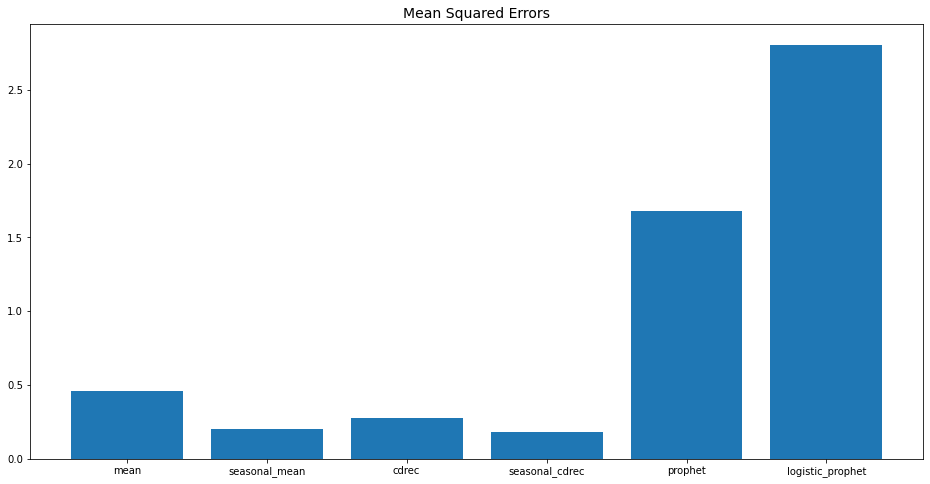
\includegraphics[width=14.4cm]{figures/impute_mse.png}
\caption{Mean Square Errors for Imputation}
\label{fig:impute_mse}
\end{SCfigure*}
\begin{SCfigure*}[\sidecaptionrelwidth][h!]
\centering
    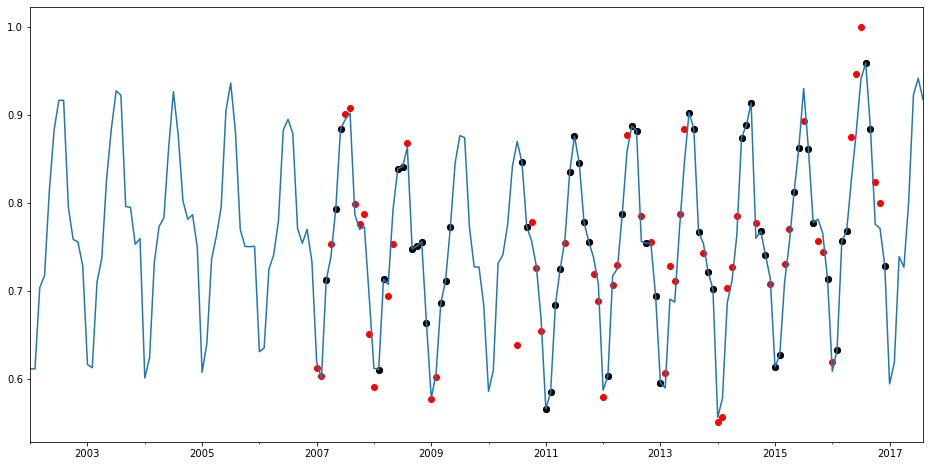
\includegraphics[width=14.4cm]{figures/impute_seasonal_cdrec.png}
\caption{Seasonal CDRec Imputation}
\label{fig:impute_seasonal_cdrec}
\end{SCfigure*}

\subsection{Model Fitting}
We fit a total of five variants of four models to the data.
We fit two baseline variants, Facebook Prophet, exponential smoothing (Holt-Winters), and SARIMA models.
The baseline models repeated either the last data point or the data point from 12 months earlier, depending on variant.
SARIMA used auto-arima methods, which include automatic differencing.
The auto-arima was used to overcome any concerns with non-stationary series.

As with imputation, we used mean square error as the metric and we scaled all time series to $[0,1]$ before fitting models.
Model fitting was validated by using the last eighth of the training timestamps as a holdout validation set.
After validation, the model was refit on the entire training set and tested on the original holdout set.
Plotted examples of fit models are shown in Fig.~\ref{fig:model_baseline_1M_zoomed} through Fig.~\ref{fig:model_sarima_zoomed}.

\begin{SCfigure*}[\sidecaptionrelwidth][h!]
\centering
    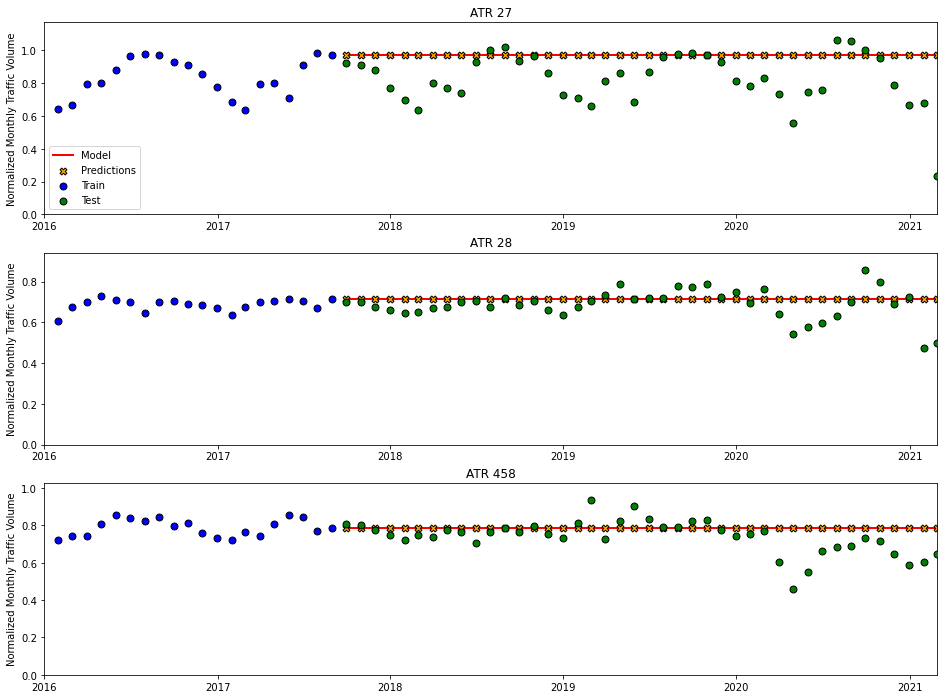
\includegraphics[width=14.4cm]{figures/model_baseline_1M_zoomed.png}
\caption{Baseline (1 month lag) Test}
\label{fig:model_baseline_1M_zoomed}
\end{SCfigure*}

\begin{SCfigure*}[\sidecaptionrelwidth][h!]
\centering
    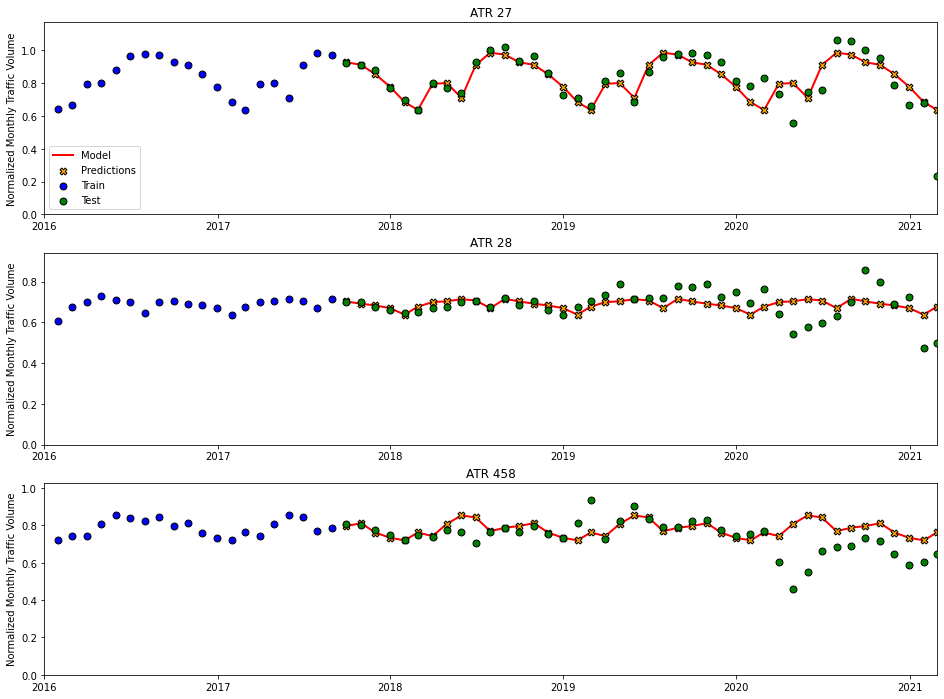
\includegraphics[width=14.4cm]{figures/model_baseline_12M_zoomed.png}
\caption{Baseline (12 month lag) Test}
\label{fig:model_baseline_12M_zoomed}
\end{SCfigure*}

\begin{SCfigure*}[\sidecaptionrelwidth][h!]
\centering
    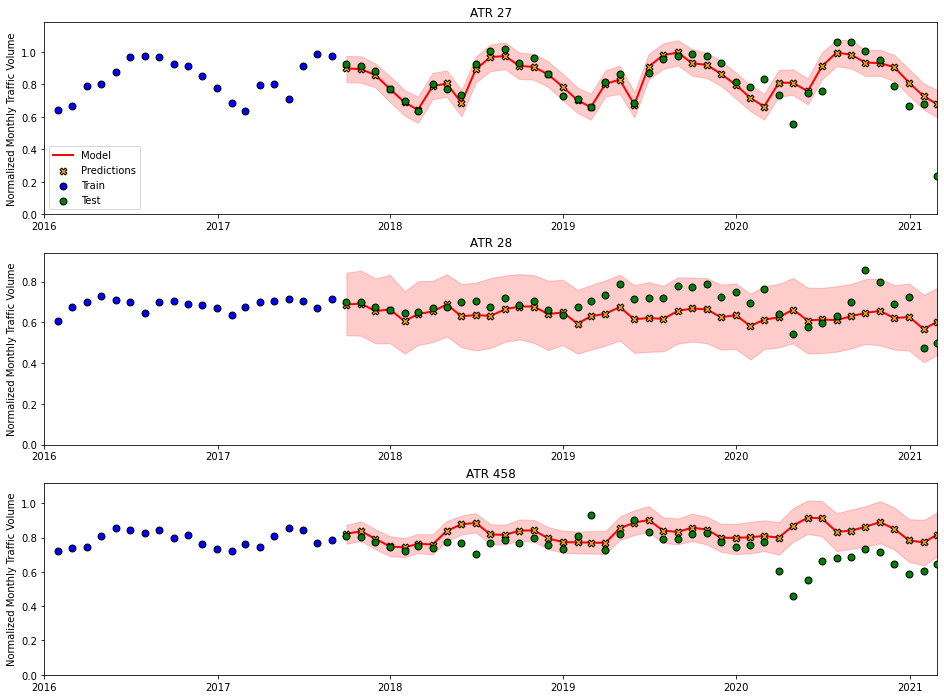
\includegraphics[width=14.4cm]{figures/model_prophet_zoomed.png}
\caption{Prophet Test}
\label{fig:model_prophet_zoomed}
\end{SCfigure*}

\begin{SCfigure*}[\sidecaptionrelwidth][h!]
\centering
    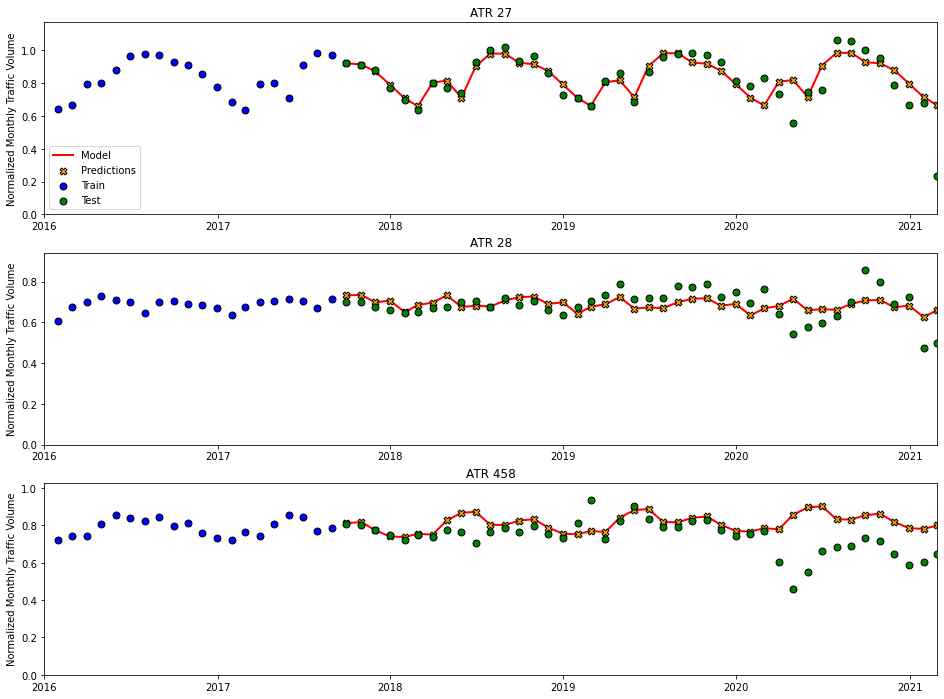
\includegraphics[width=14.4cm]{figures/model_holt_winters_model_zoomed.png}
\caption{Exponential Smoothing Test}
\label{fig:model_holt_winters_model_zoomed}
\end{SCfigure*}

\begin{SCfigure*}[\sidecaptionrelwidth][h!]
\centering
    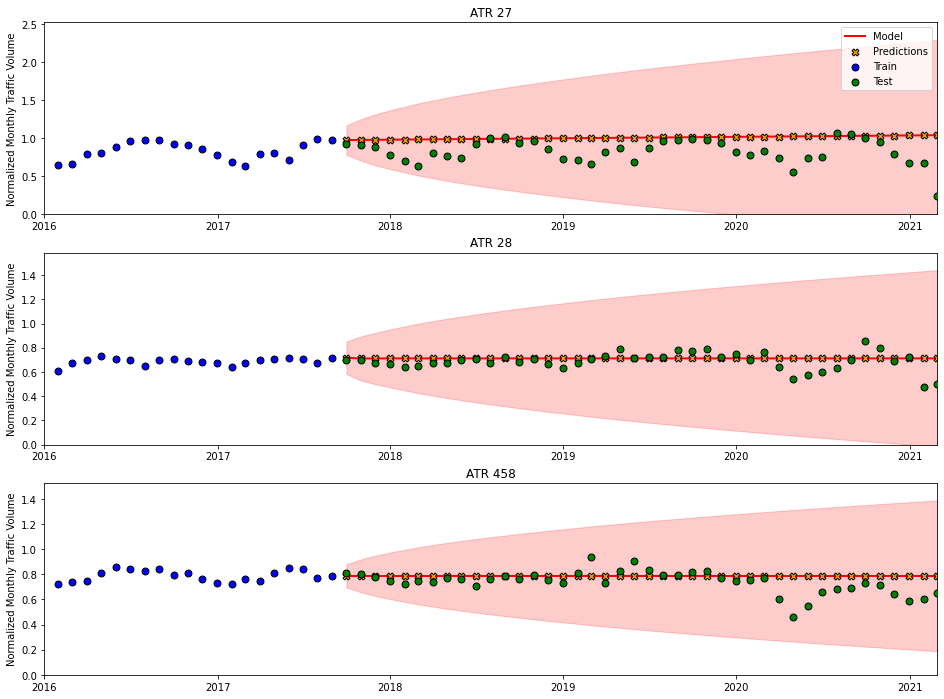
\includegraphics[width=14.4cm]{figures/model_sarima_zoomed.png}
\caption{SARIMA}
\label{fig:model_sarima_zoomed Test}
\end{SCfigure*}

We found that no model outperformed the baseline, although Prophet came close (Fig.~\ref{fig:model_mean_squared_error}).
Because of this, we did not attempt to make any future predictions.
Strangely, although drop in traffic due to the pandemic occurred entirely within the holdout set, the 12-month lag model proved a better fit.
Additionally, the SARIMA results seem particularly poor (Fig.~\ref{{fig:model_sarima_zoomed Test}}).
Further investigation is warranted into why this may be the case.

\begin{SCfigure*}[\sidecaptionrelwidth][h!]
\centering
    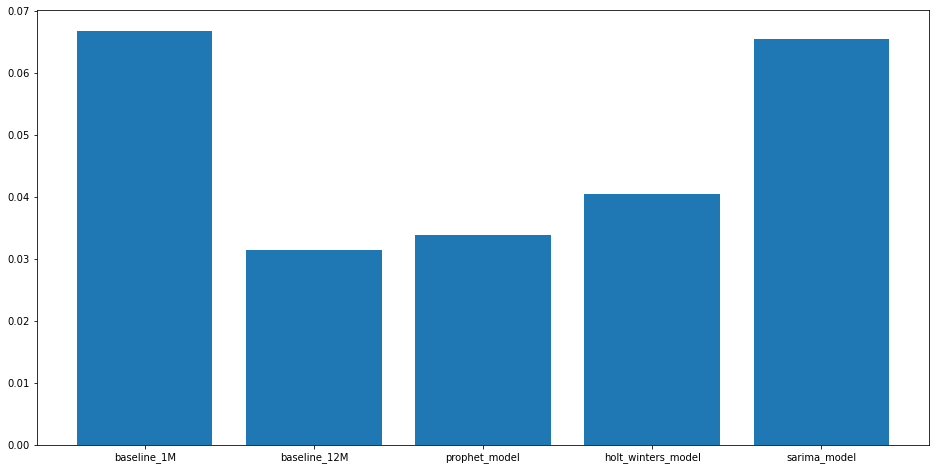
\includegraphics[width=14.4cm]{figures/model_mean_squared_error.png}
\caption{Mean Square Errors for Model Fitting}
\label{fig:model_mean_squared_error}
\end{SCfigure*}

\subsection{Future Directions}
None of the models we examined here can explicitly handle the correlation between time series.
All methods were applied to each time series independently.
There is a SARIMA derivative that includes the ability to use geographical information (STARIMA, or Space-Time Autoregressive Integrated Moving Average).
We would like to examine this or other methods to include the implicit correlation.
Deep learning methods have the ability to do this.
While working with the models described above, we also explored using plain neural networks as well as convolutional (CNN) and recurrent (RNN) versions.
Of these, the CNNs tested provided the best promise, but none outperformed even the exponential smoothing models.
The success of such models on other problems leaves hope that they can be adapted for this study as well.

%%%%%%%%%%%%%%%%%%%%%%%%%%%%%%%%%%%%%%%%%%%%%%%%%%%%%%%%%%%%%%%%%%%%%%%%%%%%%%%%%%%%%%%%%%%%%%%%%%%%%%%%%%%%%%%%%%%%%%%%
%%%%%%%%%%%%%%%%%%%%%%%%%%%%%%%%%%%%%%%%%%%%%%%%%% Bibliography %%%%%%%%%%%%%%%%%%%%%%%%%%%%%%%%%%%%%%%%%%%%%%%%%%%%%%%%
%%%%%%%%%%%%%%%%%%%%%%%%%%%%%%%%%%%%%%%%%%%%%%%%%%%%%%%%%%%%%%%%%%%%%%%%%%%%%%%%%%%%%%%%%%%%%%%%%%%%%%%%%%%%%%%%%%%%%%%%

\begin{thebibliography}{9}
    \bibitem{khayati}
    Khayati, M., Cudré-Mauroux, P. \& Böhlen, M.H.
    "Scalable recovery of missing blocks in time series with high and low cross-correlations."
    Knowl Inf Syst 62, 2257–2280 (2020).
    \url{https://doi.org/10.1007/s10115-019-01421-7}
\bibitem{mndot}
Minnesota Department of Transportation,
"MnDOT Vision"
\url{https://www.dot.state.mn.us/vision/}
No Date.
\bibitem{fhwa}
Office of Highway Policy Information, Policy and Governmental Affairs, Federal Highway Administration, United States
Department of Transportation,
"Highway Statistics 2019"
\url{https://www.fhwa.dot.gov/policyinformation/statistics/2019/}
2020.
\bibitem{fhwa2}
Office of Highway Policy Information, Policy and Governmental Affairs, Federal Highway Administration, United States
Department of Transportation,
"Traffic Monitoring Guide"
\url{https://www.fhwa.dot.gov/policyinformation/tmguide/tmg_fhwa_pl_17_003.pdf}
October 2016.



\end{thebibliography}
%%%%%%%%%%%%%%%%%%%%%%%%%%%%%%%%%%%%%%%%%%%%%%%%%%%%%%%%%%%%%%%%%%%%%%%%%%%%%%%%%
%%%%%%%%%%%%%%%%%%%%%%%%%%%%%%%%%%%%%%%%%%%%%%%%%%%%%%%%%%%%%%%%%%%%%%%%%%%%%%%%%
%%%%%%%%%%%%%%%%%%%%%%%%%%%%%%%% WARNING!!!! %%%%%%%%%%%%%%%%%%%%%%%%%%%%%%%%%%%%
%%%%%%%%%%%%%%%%%%%%%%%%%%%%%%%%%%%%%%%%%%%%%%%%%%%%%%%%%%%%%%%%%%%%%%%%%%%%%%%%%
%%%%%%%%%%%%%%%%%%%%%%%%%%%%%%%%%%%%%%%%%%%%%%%%%%%%%%%%%%%%%%%%%%%%%%%%%%%%%%%%%

% Everything below this point is the earlier capstone, imported for reference purposes so that I can compare LaTeX code.
% This should be deleted when complete.



%The report provides a row for each play (see Fig.~\ref{fig:playByPlay} for an example).
%Unlike the live feed, the HTML report gives the game strength. The report indicates the strength from the point of
%view of the team with the event, using \texttt{EV} for even-strength, \texttt{PP} for power play, and \texttt{SH}
%for short-handed.
%
%\begin{figure}[h!]
%\centering
%\includegraphics[width=\linewidth]{figures/placeholder.png}
%\caption{Shot attempts by strength}
%\label{fig:shot_attempts_by_strength}
%\end{figure}


%\section{Modeling}
%\subsection{Model Selection}

%\subsubsection{Dummy Classifiers}

%\subsection{Model Tuning}
%Having selected a model, we used cross-validation to set hyperparameters. Hyperparameters considered were the learning
%rate, maximum iterations, maximum depth, and $L_2$ regularization. The resulting selection scored approximately the
%same as the default model (see Fig.~\ref{fig:calibration_plot_best}).

%\subsection{Model Interpretations}
%\label{subsec:model_interp}
%\subsubsection{Feature Importance}

%\subsubsection{Prediction Validity}

%\section{Future Work}
%\subsection{Feature Engineering}
%The Fig.~\ref{fig:feature_importance} gives ideas for possible changes to features for modeling.

\end{document}